% Suitable Algorithm Selection

\chapter{Suitable Algorithm Selection}
Unreliable Machine Learning models can be the result of inadequate model assumptions where inappropriate or unsuitable algorithm/s have been used.
The appropriacy of an algorithm is dependant on multiple factors. One such factor is the level of supervision required, which in turn is dependant on the amount and type of data available.
Another key factor is the use case of the model and its intended outcomes. Generally model parameters are curated for specific applications and will differ to other use cases.
Therefore, it is important to make use of inductive bias\cite{saria2019tutorial} through suitable algorithm selection when developing reliable models.

In this chapter we will first train a number of models using different supervised learning algorithms before comparing respectives evaulation metrics. 
Afterwards, research will be performed on algorithm selection for other use cases before finally reccomendations are presented.

\section{Dataset \& Preprocessing}
The predictive maintenance dataset will be used again to classify failures of an ioT gadget.
During one week, maintenance data was collected from six devices every hour for 168 hrs.
Therefore, this data set contains 1008 rows of data. 
Each cycle of data reading contains the following measurements: 

% \begin{table}[H]
%     \begin{center}
%         \caption{Measurements Dataset} 
%         \begin{tabular}{ l|l } 
%          \toprule
%          \textbf{Measurement} & \textbf{Description} \\  [0.5ex] 
%          \midrule
%          \textbf{Measurement Time} & Time \\
%          \textbf{Gadget ID} & Device number \\
%          \textbf{Vibration x sensor} & Horizontal vibration \\ 
%          \textbf{Vibration y sensor} & Vertical vibration \\ 
%          \textbf{pressure sensor} & Hose pressure \\
%          \textbf{Temperature sensor} & Internal temperature \\
%          \bottomrule
%         \end{tabular}
%     \end{center}
% \end{table}

% The failures dataset contains the precise times each gadget failed. 
% During the course of the week, 105 failures were recorded.
% Device failure is to be classified when the time remaining to device failure is less than one hour.

This dataset has been split into two datasets for training and testing respectively.
The training dataset will compromise of all data collected from gadget IDs 1-4, leaving data from gadgets 5 and 6 for the test set.
This will ensure the trained models are tested on completely new data. For more information on the dataset and use case, please see \cite{ahonen}.

\section{Algorithms}
The following section shortlists and describes algorithms which can be used to train a supervised model. 
Also discussed are the factors affecting the performance and reliability of these algorithms.

\subsection{Support Vector Machines}
Support Vector Machines (SVM) is a common supervised machine learning algorithm for both classification and regression tasks.
A key attribute of SVMs is its high accuracy and precision in thge segregation of classes.
SVMs create $n$-dimensional hyperplanes to segregate datapoints into $n$ number of classes/groups. 
The algorithm aims to achieve the maximum margin between support vectors (closest points), i.e. maximise the minimum margin.

\begin{figure}[h]
    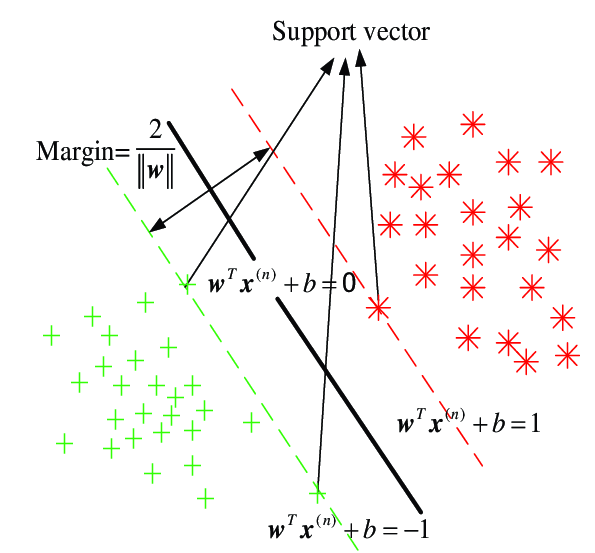
\includegraphics[scale=0.5]{Support-vector-machine-SVM-model-c-2019-IEEE-28.png}
    \centering
    \caption{Support Vector Machine \cite{svm-pic}}
    \label{fig:SVM}
\end{figure}

In the case where two classes can be linearly seperated, we consider the following as a representation of a dataset, $S$ \cite{6653952} \cite{d163fd27cc414d1a806b3e2db0164bfc}.
\begin{equation}
    S = \Big\{x_i \in \R^{1 \times p}, y_i \in \{-1, 1\}\Big\}^n_{i=1}
\end{equation}

The values $\{-1, 1\}$ represent two classes of data, $A$ and $B$,
\begin{equation}
    y_i = \begin{cases}
        1, & \text{if $i$} \text{-th sample} \in  A\\
        -1, & \text{if $i$} \text{-th sample} \in  B.
    \end{cases}
\end{equation}

The hyperplane can then be defined as $F_0$ in $\R^D$ space as,
\begin{equation}
    F_0 = \big \{x|f(x) = x \beta + \beta_0 = 0 \big \} 
\end{equation}  
where, 
$\beta \in \R^D$ with norm $||\beta|| = 1$

For a new sample $x^{new}$ which is not within dataset $S$, we can detemine a classification as,
\begin{equation}
    y_{new} = \begin{cases}
        1 \text{(Class A) }, & \text{if } f(x^{new}) > 0 \\
        -1 \text{(Class B) }, & \text{if } f(x^{new}) < 0
    \end{cases}
\end{equation}

The performance of SVMs can be further improved by implementing kernel methods. Some popular kernel functions are:
\begin{figure}[h]
    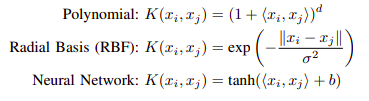
\includegraphics[scale=0.7]{SVM_kernel.png}
    \centering
    % \caption{Popular Kernel Functions \cite{6653952}}
    \label{fig:kernel}
\end{figure}

A linear kernel will be used in this experiment.

\subsection{k-Nearest Neighbours}
k-Nearst Neighbours (k-NN) is a simple supervised machine learning algorithm used in both classification and regression problems. 
This approach classifies objects based on the compuatational distances or similarities between samples/values.
The k-NN algorithm only requires tuning of a single parameter, $k$, which represents the amount of nearest samples within the neighbourhood \cite{d163fd27cc414d1a806b3e2db0164bfc}.
The choice of $k$ will affect the algorithm's performance where a value too small would create higher variance hence resulting in less stability.
A larger $k$ value will produce higher bias resulting in lower precision. 

After the number of neighbours, $k$, has been selected, the distances between the query data point, $x_q$, and an arbitrary data point, $x_i$ are to be determined.
Most commonly used is the Euclidean distance (\ref{Euclidean}), however Manhattan distance (\ref{Manhattan}) may also be applied \cite{knn}.

\begin{equation} \label{Euclidean}
    d(x_q,x_i) = \sqrt{\sum_{i=1}^{m} (x_q - x_i)^2}
\end{equation}
\begin{equation} \label{Manhattan}
    d(x_q,x_i) = \sum_{i=1}^{m} \lvert x_r - x_i \rvert
\end{equation}

The resulting values are then sorted by distance from smallest to largest and the first $k$ entries are selected. 
In classification problems, the mode of $k$ labels is returned, while the mean of $k$ labels is returned in regression problems.
The choice of parameter $k$ can impact the models reliability. Too small a value for $k$ will result in higher variance while a value too high will increase bias. 
This can be problematic when used on noisy datasets. Cross validation can be used to determine the correct $k$ value.

\subsection{Random Forest}
\label{sec:rand}
Random Forest is an ensemble machine learning method which creates multiple random decision trees and combines their respective votes (classification) or averages (regression) to improve prediction accuracy and fitting \cite{rf}.

% \enlargethispage{3\baselineskip}
% \begin{figure}[h]
%     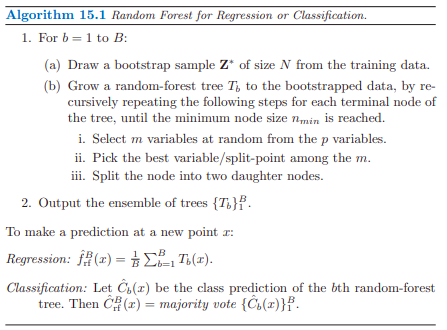
\includegraphics[scale=0.7]{random_forest.png}
%     \centering
%     \caption{Random Forest Algorithm \cite{rf}}
%     \label{fig:RF}
% \end{figure}

This algorithm is able to perform very well on huge datasets with thousands of variables. 
It is able to achieve high accuracy scores without overfitting or the need of data pruning \cite{8074494}.
The rate of error experienced in random forests can come down to a number of factors.
One such factor is the interelationshiip between any two trees within the forest. 
If the interelationship between two trees begins to increase, so will the error.
Therefore, this algorithm is able to perform better in high dimensional trees as complxity increases.
 
For extensive information on the inner workings on Random Forests, see \cite{10.5555/2503308.2343682}
A brief algorithmic overview of random forests \cite{rf} is shown below:

\begin{algorithm}[H]
    \SetAlgoLined
    \begin{enumerate}
        \item for b = 1 to B:
        \bigskip
        \begin{enumerate}
            \item Draw bootstrap sample $Z*$ of size $N$ from the training data.
            \item Develop random forest tree, $T_B$ using bootstrapped data. Continuously repeating the subsequent process at each terminal node of the tree, 
            until minimum node size, $n_{min}$ 
            \bigskip
            \begin{enumerate}
                \item Randomly select $m$ variables from $p$ variables
                \item Choose the optimal variable/split-point among the $m$ variables.
                \item Split node into two child nodes
            \end{enumerate}
        \end{enumerate}
        \bigskip
        \item Output ensemble of trees $\{T_b\}^B_1$
    \end{enumerate}

    \bigskip
    To make a prediction at new point, $x$: \\
    \\
    \textbf{Classification}: $\hat{C}_{rf}^B(x)$ = majority vote $\{\hat{C}_b(x)\}^B_1$, where $\hat{C}_b(x)$ is the class prediction of the bth random forest tree\\
    \\\textbf{Resgression}:  $\hat{f}^B_{rf}(x) = \dfrac{1}{B} \sum^B_{b=1}T_b(x)$
    \caption{Random Forest Algorithm for Classification and Regression \cite{rf}}
\end{algorithm}

\subsection{Neural Networks}
Neural Networks are a part of Deep Learning which in turn is a subset of Machine Learning.
The network is made up layers of neurons.
The first layer, the input layer, recieves input and the final layer, output layer, makes the prediction based on the computations taken place within the hidden layers.
Neurons in adjacent layers are connected via channels and are assigned a numerical weight and threshold.
If the output of any particular neuron exceeds the threshold value, that neuron is activated and data is sent to the following layer within the network.
Predictions are made based on the neuron with highest value/probability at the output layer. 
Neurwal networks are self-adaptive through forward and backward propogation using real data

When it comes to reliability it is important to consider the amount of hidden layers and the amount of neurons within.
Too few hidden layers would represent a linear problem, while additional layers create complexity hence becoming non linear \cite{4618341}.
Too few neurones would result in underfitting while too many neurons would not only cause overfitting but also significantly increase the training time.

\begin{figure}[h]
    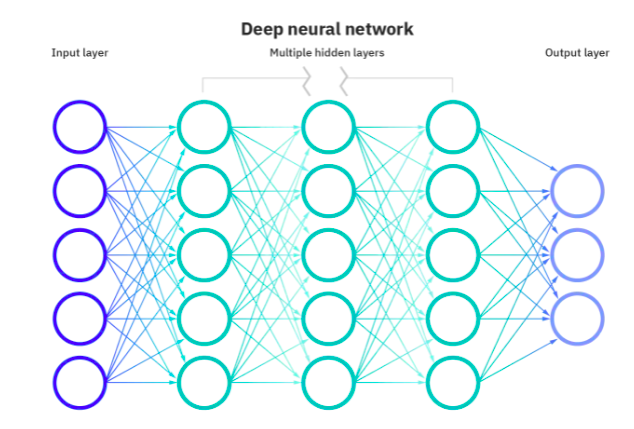
\includegraphics[scale=0.6]{neuralnetwork.png}
    \centering
    \caption{Neural Network \cite{IBM-nn}}
    \label{fig:NN}
\end{figure}

\enlargethispage{-2\baselineskip}
Mathematically represented \cite{IBM-nn}, the Neural Network follows equation (\ref{eq:nn}) and activation is dependant on equation (\ref{eq:threshold}).
\begin{equation}
    \label{eq:nn}
    \sum^m_{i=1} w_ix_i + bias = w_1x_1 + w_2x_2 + w_3x_3 + bias
\end{equation}
\begin{equation}
    \label{eq:threshold}
    \text{threshold function} = \begin{cases}
        1 & \text{if} \sum w_ix_i + bias \geq threshold\\
        0 & \text{if} \sum w_ix_i + bias < threshold
    \end{cases}
\end{equation}
where:
\begin{itemize}
    \item $x_i$ is an input
    \item $w_i$ is a weight
    \item Each neuron is assosicated with a numerical bias
\end{itemize}

\section{Experimental Results}
Building on top of the predictive maintenance project \cite{ahonen}, we train models using the following algorithms and test for Precision, Recall, Accuracy, and AUC scores.
The results are depicted in Figures (\ref{fig:Metric plot}, \ref{fig:AUC}), and Tables (\ref{table:Metrics}, \ref{table:Conf})
\begin{itemize}
    \item Random Forests (RF)
    \item Logarithmic Regression
    \item Linear Regression
    \item k-Nearest Neighbours (knn)
    \item Neural Networks (nn)
    \item Support Vector Machines (SVM)
    \item Naive Bayes
    \item Stochastic Gradient Descent (SGD/clf)
\end{itemize}

\begin{figure}[H]
    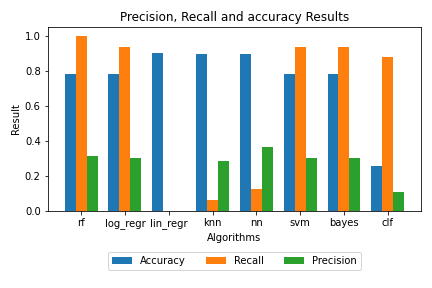
\includegraphics[scale=0.9]{results.png}
    \centering
    \caption{Precision, Recall and Accuracy Scores}
    \label{fig:Metric plot}
\end{figure}

\begin{figure}[H]
    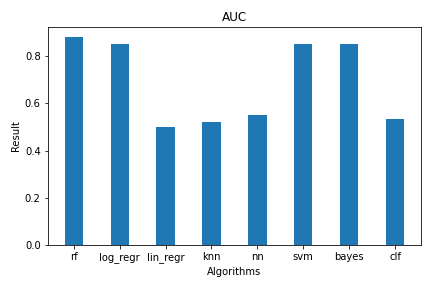
\includegraphics[scale=0.9]{AUC.png}
    \centering
    \caption{Area Under the Curve}
    \label{fig:AUC}
\end{figure}

\begin{table}[H]
    \caption{PDM Classification Metrics}
    \label{table:Metrics}
    \begin{tabular}{lrrrrr}
        \toprule
            \textbf{Algorithm} &  \textbf{Precision} &  \textbf{Recall} &  \textbf{Accuracy} &       \textbf{AUC} &        \textbf{F1} \\
        \midrule
        \textbf{Random Forest} &   0.310680 &  \cellcolor{lightgray} 1.0000 &  0.782875 &  \cellcolor{lightgray}0.879661 &  \cellcolor{lightgray}0.474074 \\
        \textbf{Logarithmic Regression} &   0.300000 &  0.9375 &  0.779817 &  0.850106 &  0.454545 \\
        \textbf{Linear Regression} &   0.000000 &  0.0000 &  \cellcolor{lightgray}0.902141 &  0.500000 &  0.000000 \\
        \textbf{k Nearest Neighbours} &   0.285714 &  0.0625 &  0.892966 &  0.522775 &  0.102564 \\
        \textbf{Neural Network} &   \cellcolor{lightgray}0.363636 &  0.1250 &  0.892966 &  0.550636 &  0.186047 \\
        \textbf{SVM} &   0.303030 &  0.9375 &  0.782875 &  0.851801 &  0.458015 \\
        \textbf{Naive Bayes} &   0.303030 &  0.9375 &  0.782875 &  0.851801 &  0.458015 \\
        \textbf{CLF} &   0.104869 &  0.8750 &  0.256881 &  0.532415 &  0.187291 \\
        \bottomrule
    \end{tabular}
\end{table}

\begin{table}[h]    
    \centering
    \caption{PDM Confusion Matrix}
    \label{table:Conf}
    \begin{tabular}{lrrrr}
        \toprule
        \textbf{Algorithm} &   \textbf{TP} &   \textbf{FP} &  \textbf{FN} &  \textbf{TN} \\
        \midrule
        \textbf{Random Forest} &  224 &   71 &   0 &  32 \\
        \textbf{Logarithmic Regression} &  225 &   70 &   2 &  30 \\
        \textbf{Linear Regression} &  295 &    0 &  32 &   0 \\
        \textbf{k Nearest Neighbours} &  290 &    5 &  30 &   2 \\
        \textbf{Neural Network} &  288 &    7 &  28 &   4 \\
        \textbf{SVM} &  226 &   69 &   2 &  30 \\
        \textbf{Naive Bayes} &  226 &   69 &   2 &  30 \\
        \textbf{CLF} &   56 &  239 &   4 &  28 \\
        \bottomrule
    \end{tabular}
\end{table}

In Table \ref{table:Metrics}, highlighted are the most optimal comparison scores between tested algorithms.
The ensemble method, Random Forests, is evidently the most suited method to this predictive maintenace application.
Linear Regression delivered the highest accuracy meaning it was able to make correct predictions the best. 
However, it did not perform well in the other metrics. 
This highlights that algorithm evaluation cannot be determined based on accuracy alone and is supported by the study \cite{8320256}.

To ensure reliability and robustness, the goals of the use case should be considered and may contradict performance metrics.
In this scenario, a True Positive (TP) case where the predicted failures are actual failures should take precedence as this is the money saving factor. 
A False Negative (FN) case occurs when the model predicts a non-failure but in reality a failure has occured. This would result in large financial penalties for the company due to downtime.
Therefore, the highest amount of TP cases and lowest amount of FN cases are desired.

\section{Further Research}

A seperate study compares existing resgression based machine learning algorithms on a similar but more complex predictive maintenance application,
\textit{'Prediction of Remaining Useful Lifetime (RUL) of Turbofan Engine using Machine Learning'} \cite{RUL}.

During this study, models were trained on a dataset obtained by NASA's data repository, where turbofan jet engines are run until failure.
During operation 21 sensor measurements are recorded against a time series per engine. Training and evaluation occurs on four datasets, each containing data from 100-250 engines. 
This dataset is much more complex than the one used in the previous experiments,
hence it is expected to see much more variance in accuracy of the tested algorithms. 


\enlargethispage{-5\baselineskip}
Listed below are machine learning algorithms used to predict RUL in this study:
\begin{itemize}
    \item Linear Regression
    \item Decision tree
    \item Support Vector Machine
    \item Random Forest
    \item K-Nearest Neighbours
    \item The K Means Algorithm
    \item Gradient Boosting Method
    \item AdaBoost
    \item Deep Learning
    \item Anova 
\end{itemize}
\bigskip

Like the Random Forest method, Gradien Boosting, AdaBoost, and Anova are also ensemble methods.


\begin{table}[h]
    \bigskip
    \caption{RUL Algorithms Root Mean Square Error values\cite{RUL}}
    \begin{figure}[H]
        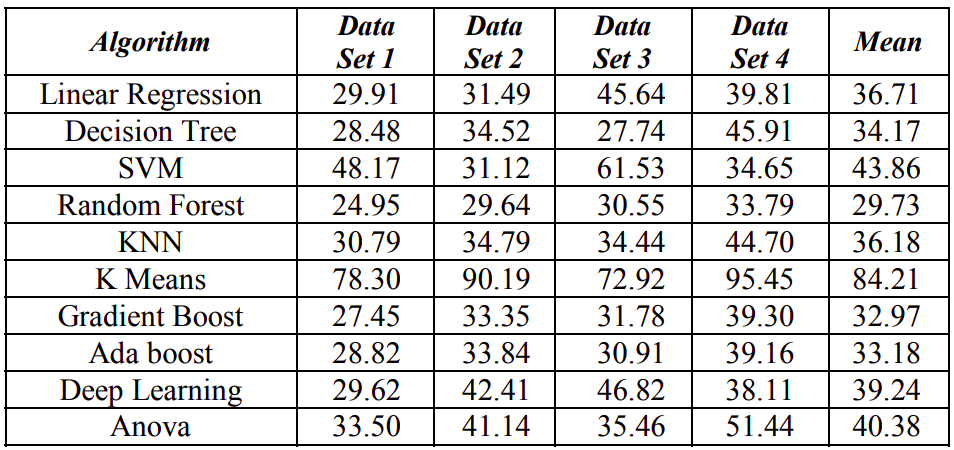
\includegraphics[scale=0.4]{RUL_results.png}
        \centering
    \end{figure}
    \label{table:RMSE}
\end{table}

\begin{figure}[H]
    \caption{RUL Algorithms Root Mean Square Error Plots per data set\cite{RUL}}
    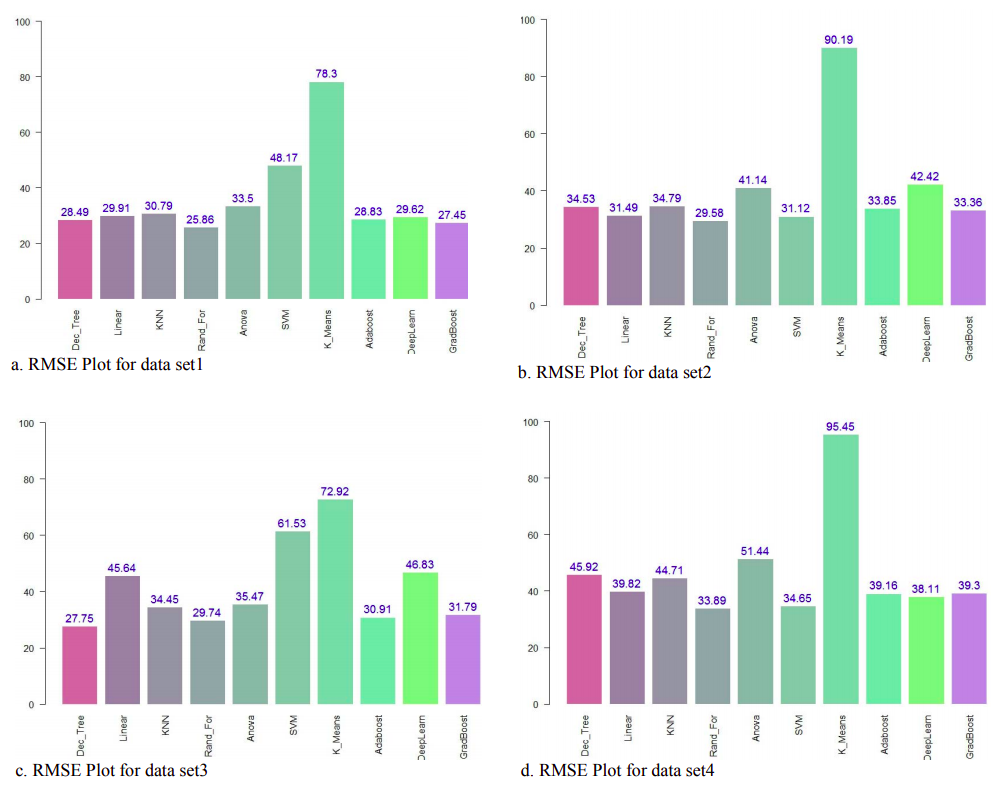
\includegraphics[scale=0.4]{RUL_RMSE.png}
    \label{fig:RMSE Plots}
\end{figure}

Table \ref{table:RMSE} and Figure \ref{fig:RMSE Plots} displays the RMSE values of all tested algorithms across all four datasets.
As can clearly be seen, the complexity of this problem results in fluctuation of evaluation scores unlike our previous classification experiment.
RMSE is a measure of the concentration of data around the line of best fit. Therefore, an algorithm with the lowest RMSE value is desired.
In this application, the random Forest algorithm produced the lowest error value.

When comparing these results to those of our previous classification experiement, it is clear that enseble methods perform the best, specifically, Random Forest. 
It should also be noted that SVM outperformed knn in the classification experiement but performed worse in the RUL regression study.

\bigskip
It is also important consider other applications of AI/ML to better understand reliability of potential algorithms.
Hence, moving away from predictive maintenance, \cite{8300383} is a study of supervised learning techniques for classification of different internal PD (partial discharge) patterns from a generator.
Analysis was conducted by considering 96 features for each PD pattern.
A total of 9 algorithms under four learning were tested where wach was tested for accuracy, ROC, precision and recall.

\begin{itemize}
    \item Functional Based Techniques
    \begin{itemize}
        \item Logistic Regression
        \item SVM
        \item Multi-layer Perceptron (MLP) - Neural Network
    \end{itemize}
    \item Probabilistic
    \begin{itemize}
        \item Naive Bayes
    \end{itemize}
    \item Decision Tree Models
    \begin{itemize}
        \item J-48
        \item Random Forest (RF)
        \item Random tree
        \item AdaBoost
    \end{itemize}
    \item Nearest Neighbours
    \begin{itemize}
        \item Instant Based-k (IBK)
    \end{itemize}
\end{itemize}

\bigskip
\begin{table}[h]
    \caption{PD Algorithms accuracy, RUC, precision and recall scores \cite{8300383}}
    \begin{figure}[H]
        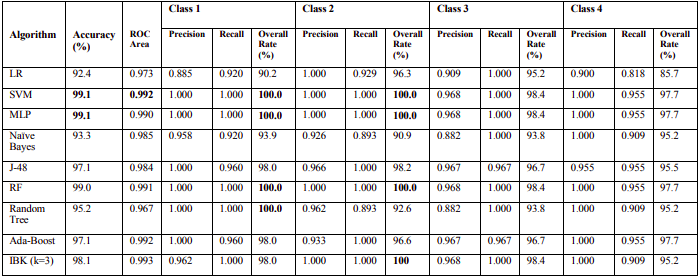
\includegraphics[scale=0.6]{PD_supervised_comparison.png}
        \centering
    \end{figure}
    \label{fig:PD_table}
\end{table}

Generally, all algorithms have performed reasonably well. However, the Functional Based Techniques outperformed other techniques in accuracy scores. 
Naive Bayes performed the worst, having the lowest accuracy score and was unable to achieve a 100\% rate in any of the four classes.


\section{Recommendations}
\subsection{Model Assumptions}
The results from previous sections highlight the importance of correct model specifications. 
Assumptions and/or expectations made in one use case most likely will not hold true in another application.
Therefore, assumptions should be refined for every use case.
A simple example provided in \cite{saria2019tutorial}, involved the illogical use of a linear model on a complex (non-linear) problem.

To aid in development of ML models, it is advised to research specific use case scenarios to find suitable algorithms through proven research into performance and reliability factors.
In \cite{pdm_review}, comprehensive research and review has been performed on machine learning methods within predictive maintenace applications.
Advantages of various algorithms have been identified in certain applications through experimentation. 
Therefore it would be beneficial to research for proven methodologies in any specific use case.  

In \cite{10.1016/j.eswa.2017.04.003}, extensive comparisons are carried out over various studies on a range of classification applications and algorithms.
Additionally, the study in, \cite{7724478}, provides advantages and disadvantages of some supervised learning techniques and suggests appropriate use cases for each algorithm.

\subsection{Ensemble Methods}
Ensemble methods are algorithms which combine multiple ML techniques to find the optimal predictive model in supervised and unsupervised ML problems.
Generally, they perform much better than single algorithms yielding higher accuracy and reliability.
The most popopular techniques used are bagging for reduction in variance, boosting for reduction in bias, and stacking to improve quality of predictions.
Comparisons between various ensemble techniques have been studied in, \cite{7340924}, \cite{8389056} and \cite{1358033}.
As alluded in Section (\ref{sec:rand}), Random Forests is an example of a bagging method. AdaBoost, as the name suggests, is a popular boosting algorithm.

\subsection{Hyperparamater Tuning}
Another recommendation for improved reliability is hyperparameter tuning/optimisation.
This can be used to aid in model design issues such as determining the appropriate number of trees in a random forest,
depth of decision tree, amount of neural network layers and the amount of neurons in the layers.
There exists many methods/algorithms for hyperparameter tuning/optimisation. 
Briefly described below are two algorithms, Bayesian Optimisation \cite{7900023} and Hyperparameter Optimisation Machines (HOM) \cite{7796889}.

\begin{algorithm}[H]
    \SetAlgoLined
    \KwIn{Initial observation $D \equiv \{x_{1:p},y_{1:p}\}$}
    \KwOut{$\{x_n^*,y_n^*\}^T_{n=1}$}
    \For{$n = 1,2,...,T$}{
         Find $x_n^* = arg max_x \EX(I(x) | GP(D))$ of (11)\\
        Calculate objective function: $y_n^* = f(x_n^*)$\\
        Enhance observation set $D = D \cup (x_n^*,y_n^*)$
    }
    \caption{Brief Bayesian Optimisation Algorithm \cite{7900023}}
\end{algorithm}

\begin{algorithm}[H]
    \SetAlgoLined
    \KwIn{Hyperparamater space $\Lambda$ observation history $\mathcal{H}$, transfer function $\mathcal{L}$, 
    acquisition function a, surrogate model $\Psi$, tradeoff parameter $\alpha$, hyperparam response function $f$ (minimisation operation)
    total HOM iterations $T$}
    \KwOut{Most optimal hyperparameter configuration}
    $\Lambda \leftarrow \emptyset, f-{best} \leftarrow \infty$\\

    \ForAll{$t = 1,...,T$}{
        \text{ Update: Fit }$\Psi$ to $\mathcal{H}$ \\
        Predict: $\lambda \leftarrow \text{arg }min_{\lambda\prime \in^\Lambda}(1 - \alpha_t) $
        $\mathcal{L}(\lambda\prime,\Lambda{t-1})-\alpha_ta (\lambda\prime\Psi)$\\
        $\Lambda_t \leftarrow \lambda_{t-1} \cup \{\lambda\}$ \\
        Calculate $f(\lambda)$ \\
        $\mathcal{H} \leftarrow \mathcal{H} \cup \{(\lambda, f(\Lambda))\}$ \\
         \\
        \If{$f(\lambda) < f_{best}$}{
            $\lambda_{best}, f_{best} \leftarrow \lambda, f(\lambda)$ 
        }
    }
    \Return{$\Lambda_{best}$}
    
    \caption{Hyperparamater Optimisation Machines (HOM) }%\cite{7796889}}
\end{algorithm}

\subsection{Evaluation Metrics}
It is also important to select appropriate evaluation metrics based on the model type and application.
As observed in our earlier experiment in section (\ref{table:Metrics}), accuracy alone cannot be used to evaluate a model's reliability and performance.
Accuracy is the fraction value of correct predictions made but does not indicate the relationships between other attributes of the model \cite{8320256}.
A Confusion Matrix is an N x N matrix specifying True Positives (TP), True Negatives (TN), False Positive (FP) and False Negative (FN) instances within the model.
Other metrics can be derived using the confusion matrix \cite{8320256}.
Depending on the specific use case, a weight or cost can be assigned to each output of the confusion matrix to indicate importance.
Table (\ref{table:Evaluation Metrics}) below is a non-exhaustive list of some common evaluation metrics for supervised learning models.
For evaluation metrics on unsupervised learning models, see \cite{palacioniño2019evaluation}.

\begin{landscape}
    \begin{table}[H]
        \centering
        \caption{Supervised Learning Evaluation Metrics}
        \label{table:Evaluation Metrics}
        \begin{tabular}{|l|c|l|}
            \hline
            \textbf{Metric}   & \textbf{Equation} & \textbf{Description} \\ \hline
            \multicolumn{3}{|l|}{\textbf{Classification:}} \\ \hline
            \multirow{2}{*}{Accuracy} &  \multirow{2}{*}{$\dfrac{TN+TP}{TN+TP+FP+FN}$   }    &  \multirow{2}{*}{Number of correct predictions made}           \\ 
            & & \\ \hline
            \multirow{2}{*}{Precision} &  \multirow{2}{*}{$\dfrac{TP}{TP+FP}$}    &  \multirow{2}{*}{Rate of positive predictions that were infact positive}           \\ 
            & & \\ \hline
            \multirow{2}{*}{Recall} &  \multirow{2}{*}{$\dfrac{TP}{FN+TP}$}    &  \multirow{2}{*}{Proportion of correctly classified positive cases }           \\ 
            & & \\ \hline
            \multirow{2}{*}{Specifity} &  \multirow{2}{*}{$\dfrac{TN}{TN+FP}$}    &  \multirow{2}{*}{Number of correct negatice predictions}           \\ 
            & & \\ \hline
            \multirow{2}{*}{F1 Score} &  \multirow{2}{*}{$\dfrac{2\cdot Precision \cdot Recall}{Precision + Recall}$}    &  \multirow{2}{*}{Harmonic mean of precision \& recall}           \\ 
            & & \\ \hline
            \multicolumn{3}{|l|}{\textbf{Regression:}} \\ \hline
            \multirow{3}{*}{Root Mean Squared Error} &  \multirow{3}{*}{$\sqrt{\dfrac{\sum^N_i=1(Predicted_i-Actual_i)^2}{N}}$}    &  \multirow{3}{*}{How well regression line fits data points}           \\ 
            & & \\ 
            & & \\ \hline
            \multirow{3}{*}{R Squared} &  \multirow{3}{*}{$1 - \dfrac{MSE(model)}{MSE(baseline)}$}    &  \multirow{3}{*}{Compares model to basic mean value}           \\ 
            & & \\
            & & \\ \hline
            \multirow{3}{*}{Adjusted R Squared} &  \multirow{3}{*}{$1-(1-R^2)\Bigg[\dfrac{n-1}{n-(k+1)}\Bigg]$}    &  \multirow{3}{*}{Adjusts to changing features}           \\ 
            & & \\
            & & \\ \hline
        \end{tabular}
    \end{table}
\end{landscape}